\chapter{Introduction to Semiconductor Based Electron Spin Qubits}
\label{chap:motivation}
\section{Qubit}
A qubit, or generally speaking a quantum mechanical two level system 
$ \ket{\Psi} = \alpha \ket{0} + \beta \ket{1} $, where $\alpha, \beta \in \mathbb{C}$ and $|\alpha|^2 + |\beta|^2=1$ can be expressed as
\begin{equation}
    \ket{\Psi}=\cos \left( \frac{\theta}{2} \right) \ket{0} + \exp(i \phi) \sin \left( \frac{\theta}{2} \right) \ket{1} \quad \text{where}\;  \phi, \theta \in \mathbb{R}
\end{equation}
when a global phase is neglected. This allows us to visualize this pure state as a point on the so called Bloch Sphere.

However, information about the exact quantum mechanical state can be lost to the environment leading to the definition of mixed states.  Mixed states are statistical ensembles of different quantum states and can be expressed via the density matrix 
\begin{equation}
    \dm = \sum_i p_i \ket{\psi_i}\bra{\psi_i}
\end{equation}
For a 2-dimensional system we can use the Pauli-Matrices to rewrite $\dm$ in terms of $\px$, $\py$ and $\pz$
\begin{equation}
    \dm= \frac{1}{2}(\eye+\vsym{r} \cdot \vecsig)
\end{equation}
where $|\vsym{r}|\le 1$. In fact $|\vsym{r}|= 1$ only for pure states and $|\vsym{r}|< 1$ for mixed states. \cite{Feynman1957}

 \begin{figure}[htbp]\centering
     \centering
     
\includegraphics[width=0.35\textwidth]{./pictures/dummy}
     \caption{PICTURE BLOCH SPHERE}
     \label{fig:bloch_sphere}
 \end{figure}

Ignoring interactions with the environment for now, we can model the time evolution of a quantum mechanical system, and therefore a qubit, using the unitary time evolution operator $U(t,t_0)$. $U$ acts on the initial state of the system given by $\ket{\psi_0}$ leading us to, $\ket{\psi(t,t_0)}=U(t,t_0)\ket{\psi_0}$, the state at the time $t$. Using the Hamiltonian $H(t)$ we can calculate $U(t,t_0)$ 
\begin{equation}
U(t,t_0)=\mc{T}\exp \left( - \frac{i}{\hbar} \int_{t_0}^t H(t') dt'  \right),
\end{equation}
using the time-ordering operator. 
For qubits the time evolution can in general be explained by rotations on the Bloch sphere, making for a very intuitive picture of qubit operations. Many of these concepts have been in use for some in NMR experiments, but can be easily applied to all kinds of qubits be it semiconductors, superconductors, NV centers or ion traps.

For two qubits, however, this simple picture breaks down. Of course we can express the individual qubits on their respective Bloch spheres, but since the interaction between the two becomes important, this can not depict the full information of the system. MORE?

\section{Quantum Dots}
Quantum dots are the predominant way to create semiconductor based qubits. A quantum dot is a system confining electrons in all the directions.

Confinement in one direction is usually archived by the growth of suiting heterostructures such as AlGaAS-GaAs or Si-SiGe combination (see REF) forming a two dimensional electron gas. Confinement in the remaining two directions is achieved by placing gate electrodes on top of the heterostructure. These allow for the creation of quantum dots, as well as for the control of tunneling to source and drain regions within the 2DEG. Further, so called plunger gates can shift the chemical potential of the quantum dot effectively controlling its population.

Interesting characteristics arise when the transport through a quantum dot is measured as a function of the plunger gate voltage. Assuming that the tunnel barriers to source and drain are clearly defined and transparent enough to allow for tunneling on a realistic timescale transport can be observed whenever one of the discrete dot energy levels is between the source and drain chemical potential. This assumes that a small bias voltage is applied between source and drain. Sweeping the gate voltage will lead to a oscillatory behaviour of the current REF. 

Since the energy levels of the dot are not only sensitive to changes in the gate voltage but also to charges nearby a quantum dot can be used as a very sensitive means of measuring charge REF. A quantum dot used in this capacity is often referred to as sensing dot or single electron transistor (SET). 

\begin{figure}[htbp] 
  \centering
     \subfigure[]{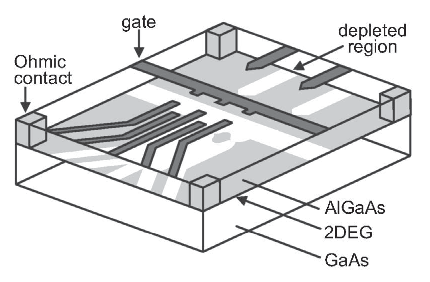
\includegraphics[width=0.49\textwidth]{./pictures/quantumdot1}}
   \subfigure[]{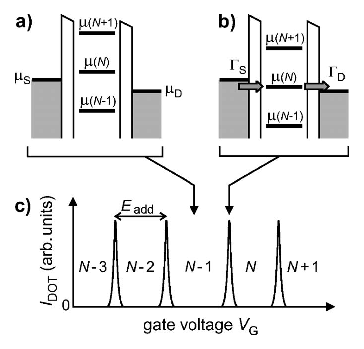
\includegraphics[width=0.49\textwidth]{./pictures/QuantumDot}}
  \caption{}
  \label{fig:quantumdots}
\end{figure}

 
\section{Heterostructure}
The heterostructures we use for our experiments is shown in PICTURE. They consist of a GaAs substrate on top of which a $\algaas \ $ layer is grown by molecular beam epitaxy (MBE). This layer contains Si-doping which provides charge carriers. These carriers accumulate at the $\algaas$/GaAs interface, where due to the band offset of the two materials a triangular quantum well is formed. The electron in this well create a two dimensional electron gas (2DEG) since they are confined in growth direction. 
The 2DEG is contacted by gold/germanium ohmic contacts which are fabricated in the Helmholz Nano Facility \cite{HNF}. This allows for control of the electrochemical potential of the 2DEG.
The heterostructure is topped off with a thin GaAs cap, on top of which metal electrodes are fabricated by electron beam lithography
These so called gates can be used to deplete the 2DEG selectively underneath the pattern by applying negative bias voltages. A possible gate design is shown in PICTURE.This procedure allows for the precise creation of dot regions with good control of the electron population within the dots.

\begin{figure}[htbp]\centering
     \centering
     \includegraphics[width=0.50\textwidth]{./pictures/Heterostructure}
     \caption{PICTURE Heterostructure}
     \label{fig:bloch_sphere}
 \end{figure}
 

\section{S-T0 Qubits}
The original proposal from Loss and DiVincenzo used individual spins in a semiconductor heterostructure as qubits. While viable for example in Silicon, this approach has a couple of inherent disadvantages in GaAs mainly caused by the perturbations due to the nuclear spin bath surrounding the qubits.
This problem can be mitigated using a double quantum dot with two spins in a external magnetic field, where the $m_z=0$ subspace of the system is used for computation. This approach has been successfully employed in many experiments and is proven to reach long coherence times in excess of $200\;\mr{\mu s}$.
Additional advantages are the option to control the qubit all electrically be changing the detuning and thus the exchange interaction between the two spins.
Straightforward spin to charge conversion.
MORE ADVANTAGES AND DIFFERENCES
200 mus Time
Single Shot Readout
Universal Control
Two  Qubit Gates 
DiVincenzo Criteria Backref





For an $\sts$ qubit the gates are used to form a double well potential, trapping exactly two electrons. An additional external magnetic field of the order of a couple $\si{100.mT}$ is applied in plane, separating of the $m_z=\pm1$ states $\ket{T_+}=\uu$ and $\ket{T_-}=\dd$ energetically. The remaining states in the $m_z=0$ subspace are then used as the computational basis states REF
\begin{align}
    \ket{0}&=\ket{S}=\frac{1}{\sqrt{2}}(\ud-\du) \\
    \ket{1}&=\ket{T_0}=\frac{1}{\sqrt{2}}(\ud+\du).
\end{align}
The degeneracy between the two computational states is lifted on the one hand by the exchange interaction $J$ and on the other hand by the magnetic field difference $\dbz$ between the dots.
$\dbz$ arises from the electron spins within the GaAs. Naturally these would cause a random difference in the magnetic field at the dot locations. However by using controlled spin flips the magnetic field gradient can be tuned to be within a few MHz of the desired values. Nevertheless control of $\dbz$ remains slow and the nuclear spins have to be "pumped" repeatedly in between measurements as the only remain stable for short amounts of time due to diffusion REFS.

The exchange interaction $J$ gives the second control axis for \sts qubits. It can be controlled via the detuning between two dots which is directly related to the voltage applied to the gate electrodes. Empirically, a exponential dependence
\begin{equation}
    J(\eps)=J_0 \exp \left( \frac{\eps}{\eps_0} \right)
\end{equation}
has been found to best describe the relation of the exchange interaction and the detuning. The resulting Hamiltonian for one qubit is then given by 

\begin{equation}
    H=\frac{\hbar J(\epsilon)}{2}\sigma_z + \frac{\hbar B_z}{2} \sigma_x.
\end{equation}

Using these two control axes universal control of \sts qubits in GaAs has been shown. A basic control cycle is depicted in \rfig{fig:controlcycle}. 

\begin{figure}[htbp]\centering
     \centering
     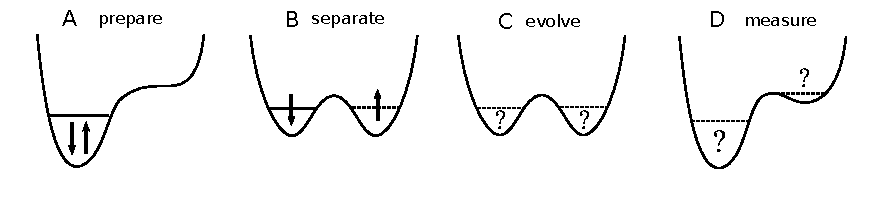
\includegraphics[width=1\textwidth]{./pictures/computationalcycle}
     \caption{PICTURE BLOCH SPHERE}
     \label{fig:controlcycle}
 \end{figure}

\begin{figure}[htbp] 
  \centering
     \subfigure[]{
\includegraphics[width=0.49\textwidth]{./pictures/dummy}}
     \subfigure[]{
\includegraphics[width=0.49\textwidth]{./pictures/dummy}}
   
  \caption{}
  \label{fig:cable}
\end{figure}


\section{Exchange Only Two Qubit System}
In theory the number of quantum dots which can be placed next to each other is only limited by fabrication. 

\begin{figure}[htbp]\centering
     \centering
     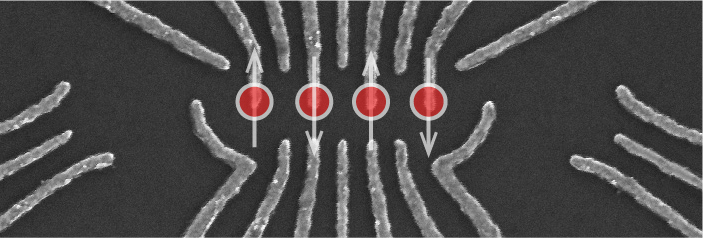
\includegraphics[width=.5\textwidth]{./pictures/gl005_SEM_electrons_small}
     \caption{PICTURE BLOCH SPHERE}
     \label{fig:controlcycle}
 \end{figure}
 
Computational Subspace

Coherent Leakage

Possible Gate design



\section{Previous Work}
\subsection{Single Qubit Gates}

Masterarbeit Pascal

PRL Paper

Bootstrap Tuning Paper

\subsection{Experimental Work on Two Qubit Gates in GaAs}

Harvard work on capacitivly coupled Qubits




